\documentclass[10pt]{beamer}

\usetheme[progressbar=frametitle]{metropolis}
\usepackage{appendixnumberbeamer}
\usepackage[numbers,sort&compress]{natbib}
\bibliographystyle{plainnat}

\usepackage{booktabs}
\usepackage[scale=2]{ccicons}
\usepackage{multicol}
\setlength{\columnsep}{1cm}

\usepackage{xspace}
\newcommand{\themename}{\textbf{\textsc{metropolis}}\xspace}

\title{Data-driven Birdstrike Risk Estimation}
% \subtitle{Subtítulo}
% \date{\today}
\date{}
\author{\textbf{Alessandro Minervini}\protect \\ Relatori: Prof. Andrew D. Bagdanov, Prof. Fabio Schoen \protect \\ Correlatore: Ing. Walter Nunziati}

\institute{Università degli Studi di Firenze \\ Scuola di Ingegneria\\ Ingegneria Informatica}
\titlegraphic{\hfill
\includegraphics[height=1.8cm]{img/logo-unifi.png}}

\begin{document}

\maketitle

\begin{frame}{Contenuti}
  \setbeamertemplate{section in toc}[sections numbered]
  \tableofcontents[hideallsubsections]
\end{frame}

\section{Introduzione}

\begin{frame}[fragile]{Introduzione}
\textbf{Wildlife strike} è l'impatto violento di un animale o più frequentemente stormi di uccelli (\textbf{birdstrike}) con un aereo.

\textbf{Cause}:
\begin{itemize}
    \item Incremento del numero di voli 
    \item Aeroporti luoghi attrattivi e di grande concentrazione per gli animali
\end{itemize}

\textbf{Conseguenze}:
\begin{itemize}
    \item Pericolo per i passeggeri
    \item Costi onerosi (riparazioni, ritardi, prevenzione)
\end{itemize}
\end{frame}

\begin{frame}{Introduzione}
%ENAC (Ente Nazionale per l'Aviazione Civile) ha adottato, come previsto dalla circolare APT-01B, il Birdstrike Risk Index version 2 (\textbf{BRI\textsubscript{2}}) per misurare il rischio di birdstrike negli aeroporti Italiani.
ENAC ha adottato\footnote{come previsto dalla circolare APT-01B} il Birdstrike Risk Index version 2 (\textbf{BRI\textsubscript{2}}) per misurare il rischio di birdstrike negli aeroporti Italiani.

Il \textbf{BRI\textsubscript{2}}:
\begin{itemize}
    \item \`E un indice mensile
    \item Identifica il rischio di un dato aeroporto
    \item Fornisce un valore di rischio tra 0 e 2 (0.5 soglia di attenzione)
    \item Si basa sull'abbondanza media delle specie, il numero di impatti per specie ed i loro effetti.
\end{itemize}
%Il lavoro di tesi è stato possibile grazie al dataset fornito da Birdcontrol S.r.l. che comprende 10+ anni di monitoraggio negli aeroporti Italiani.
\end{frame}

\begin{frame}{Introduzione}
Grazie al dataset fornito da Birdcontrol Italy S.r.l. (10+ anni di monitoraggio negli aeroporti Italiani) abbiamo:% condotto \textbf{un'analisi sul BRI\textsubscript{2}} per verificare:
\begin{itemize}
    \item \textbf{Analizzato} il BRI\textsubscript{2}
    \item \textbf{Implementato} un modello Data-driven 
    %\item Correlazione con gli eventi di birdstrike 
\end{itemize}
\end{frame}


\section{Analisi BRI\textsubscript{2}}

\begin{frame}{Analisi BRI\textsubscript{2}}
\textbf{Formula BRI\textsubscript{2}}:

\begin{itemize}
    \item \textbf{GF\textsubscript{i}} è chiamato il fattore di gruppo {{\scriptsize\begin{equation}\label{GF}
GF_i=\overline{W_i}\cdot Ag_i \cdot\frac{BS_i}{TFN} \cdot EOF_i ^{95}\end{equation}}\small}
    \item \textbf{GSR\textsubscript{i}} il fattore di rischio {{\scriptsize\begin{equation}\label{GSR}
GSR_i=\frac{GF_i}{\sum_{i=1}^{N}GF_i}\cdot DB_i
\end{equation}}\small}
    \item \textbf{BRI\textsubscript{2}} il valore finale di rischio calcolato {{\scriptsize\begin{equation}\label{BRI2_f}
BRI_2=\left(\frac{\sum_{i=1}^{N}GSR_i \cdot DF}{\overline{TFN}}\right)
\end{equation}}\small}
\end{itemize}

\textbf{Parametri critici:}
\begin{itemize}
    \item \textbf{BS\textsubscript{i}} paramentro cumulativo non mediato nel tempo
    \item \textbf{EOF\textsubscript{i}} incrementa il contributo di \textbf{BS\textsubscript{i}}
    \item \textbf{Ag\textsubscript{i}} paramentro mediato nel tempo, perdita di sensibilità degli avvistamenti
    \item \textbf{BRI\textsubscript{2}} soggetto alla perdita di sensibilità dovuto al parametro \textbf{Ag\textsubscript{i}}.
\end{itemize}
\end{frame}

\begin{frame}{Analisi BRI\textsubscript{2}}
\textbf{BRI\textsubscript{2}} per l'aeroporto di \textbf{Firenze}:
\begin{figure}
	\centering
	\fbox{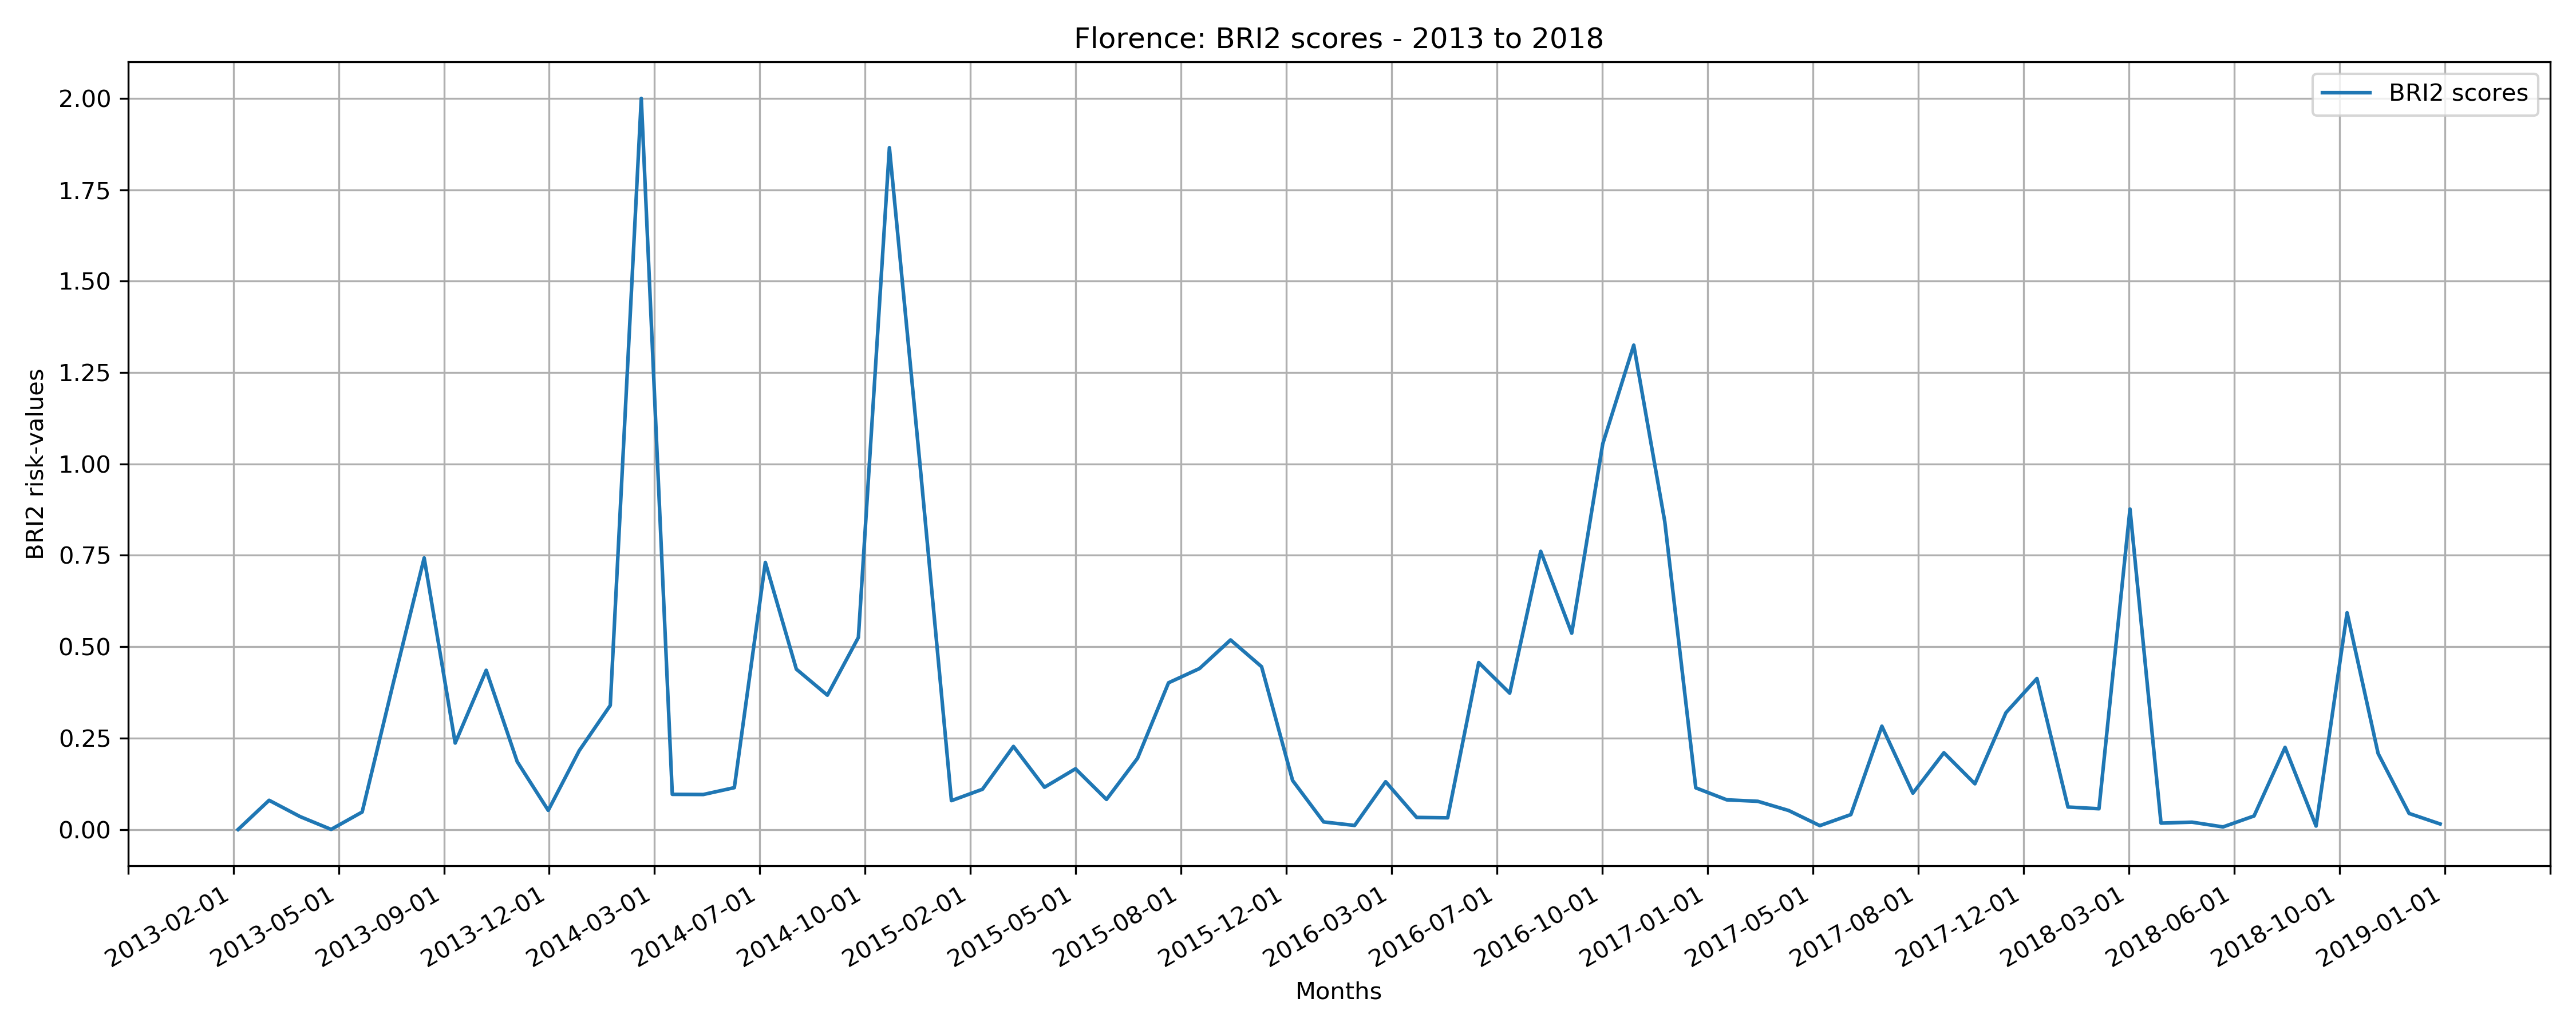
\includegraphics[width=\textwidth]{img/corr_curve_2.png}}
\end{figure}
\end{frame}

\begin{frame}{Analisi BRI\textsubscript{2}}
\textbf{BRI\textsubscript{2}} per l'aeroporto di \textbf{Firenze}:
\begin{figure}
	\centering
	\fbox{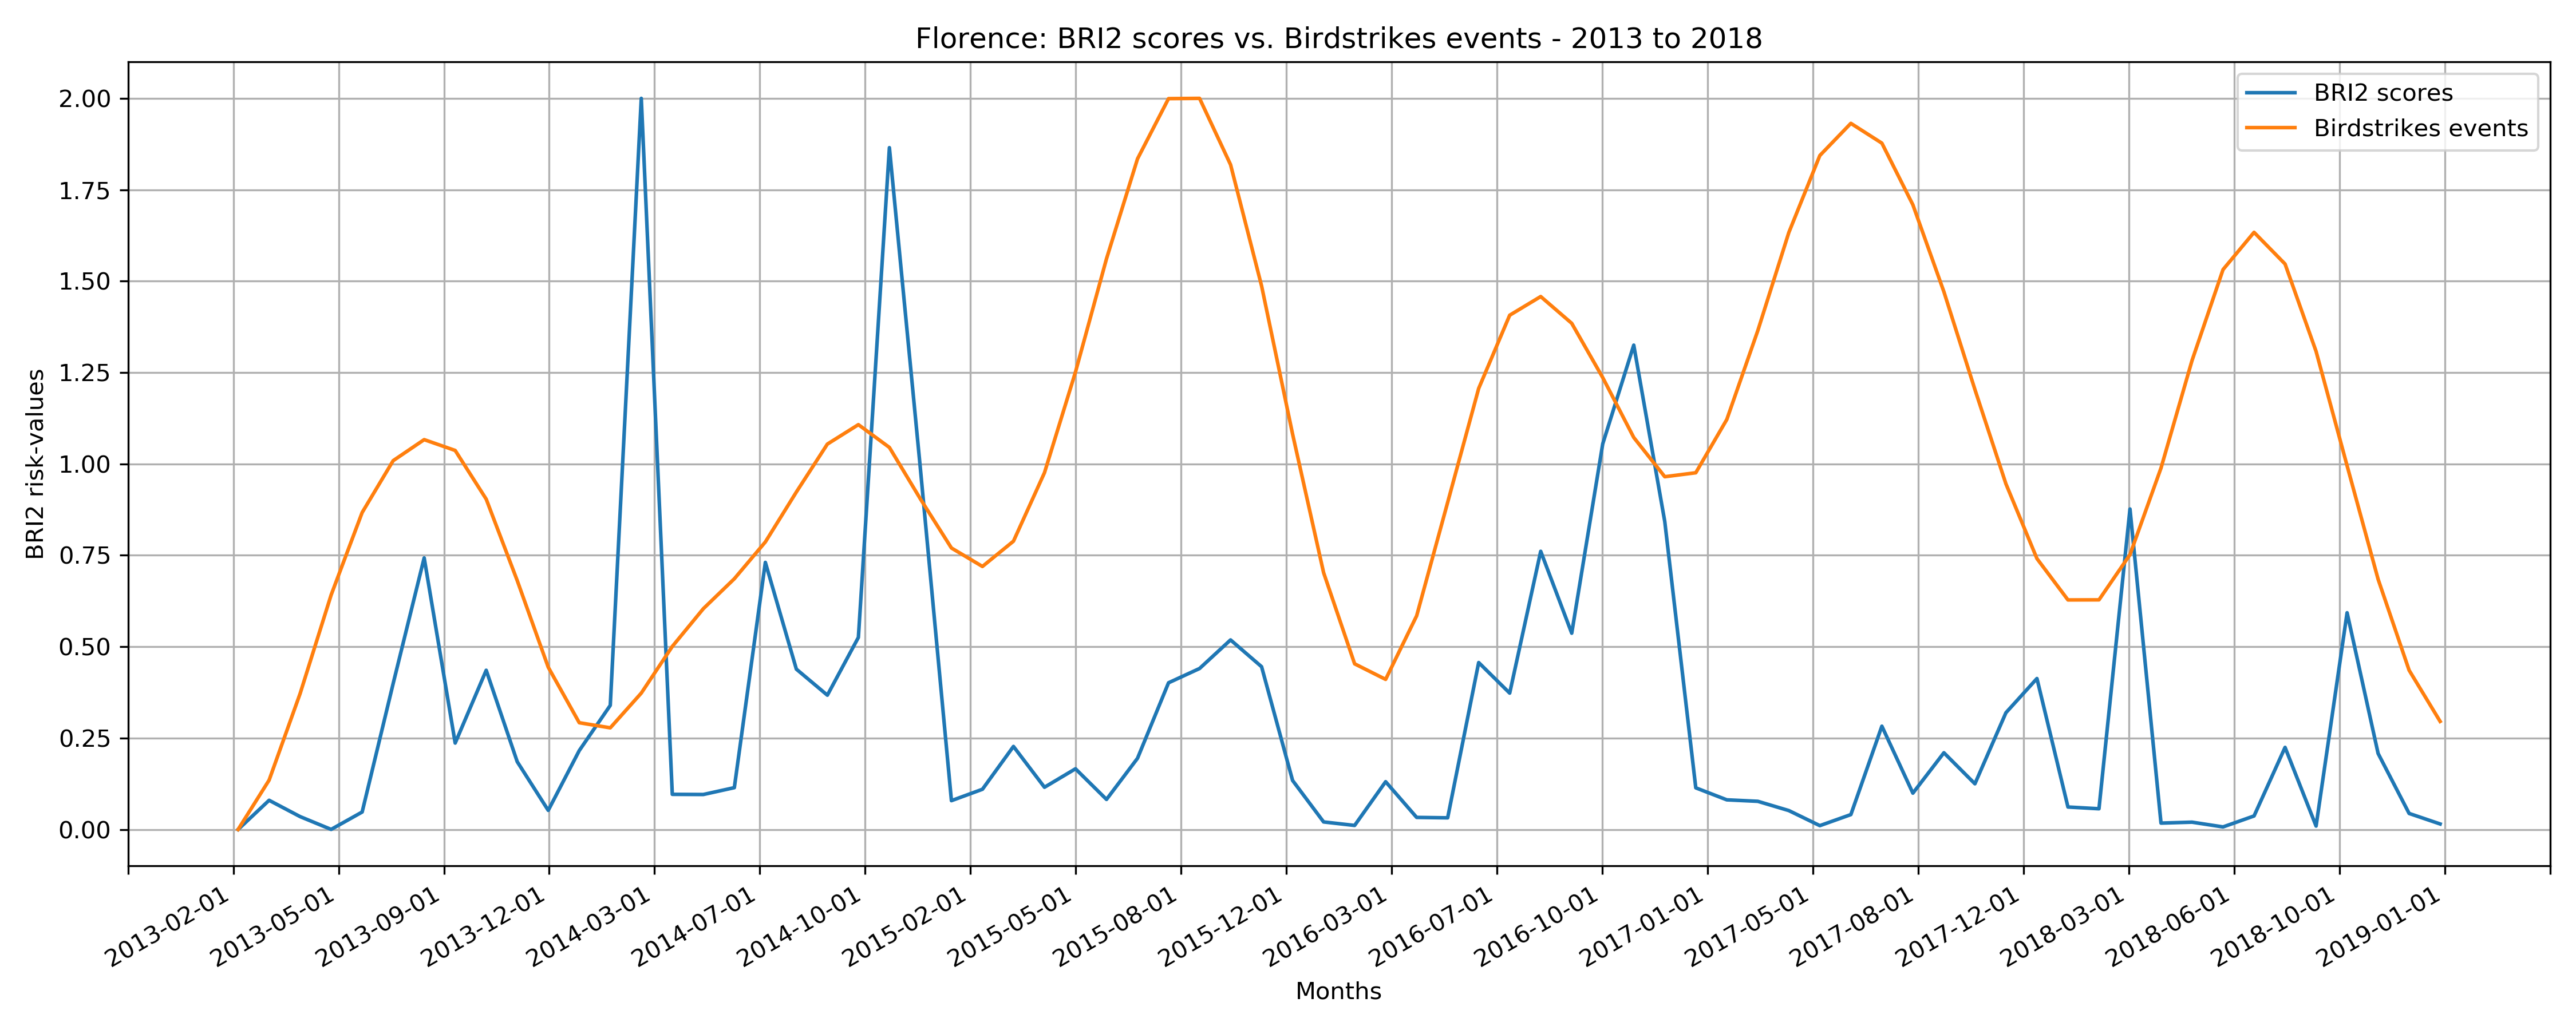
\includegraphics[width=\textwidth]{img/corr_curve_.png}}
\end{figure}
\end{frame}


\begin{frame}{Analisi BRI\textsubscript{2}}
\textbf{Correlazione} del BRI\textsubscript{2} con gli eventi di birdstrike reali:
\begin{table}
	\centering
	\scalebox{1}{
	\begin{tabular}{@{}ccc@{}}
		\toprule
		Airport & Spearman correlation \\	\midrule
		Firenze & 0.17 \\
		Pisa & 0.47 \\
		Bologna & 0.26\\
		Milano-Malpensa &  -0.14 \\
		Milano-Linate & -0.28 \\
		Verona & 0.60 \\
		Catania & 0.49 \\
	    Brescia & 0.31 \\	\bottomrule
	\end{tabular}}
\end{table}
\end{frame}

\begin{frame}{Analisi BRI\textsubscript{2}}
\textbf{Dopo l'analisi si è riscontrato che il BRI\textsubscript{2}:}
\begin{itemize}
    \item \textbf{Perde sensibilità} agli avvistamenti nel corso del tempo
    \item \textbf{\`E fortemente dipendente} da $BS_i$ creando un ranking tra le specie, indipendente dagli avvistamenti
    \item \textbf{Non correlato} con gli eventi di birdstrike storicamente accaduti
\end{itemize}
\end{frame}

\section{Modello Data-driven}

\begin{frame}{Modello Data-driven}
Il nostro modello ideale dovrebbe essere:
\begin{itemize}
    \item Un \textbf{affidabile} predittore di rischio
    \item Un indice di rischio \textbf{fortemente correlato} agli eventi di birdstrike
    \item Un indice rischio \textbf{giornaliero}, che predica il rischio osservando i giorni precedenti
\end{itemize}
%Il dataset utilizzato comprende 10+ anni di monitoraggio negli aeroporti Italiani, fornito da Birdcontrol Italy S.r.l.
\end{frame}

\begin{frame}{Modello Data-driven}

Abbiamo quindi implementato un modello:
\begin{itemize}
    \item Addestrabile per ogni aeroporto
    \item Che predice il rischio giornaliero di birdstrike futuri
    \item Basato su una finestra di osservazione di 15 giorni
\end{itemize}

Data la quantità dei dati disponibili per gli areoporti Italiani
abbiamo utilizzato tecniche di \textbf{Machine Learning supervisionato}.

\end{frame}

\begin{frame}{Modello Data-driven}
\textbf{Features scelte}:
\begin{itemize}
    \item Numero di avvistamenti per specie
    \item Condizioni meteorologiche
    \item Temperatura
    \item Intensità e direzione del vento
    \item Distanza dell'avvistamento dalla pista
    \item Ambiente di avvistamento
    \item Presenza suolo bagnato
    \item Numero di Birdstrike dei giorni della finestra di osservazione (per l'anno corrente e precedente)
\end{itemize}
Tutte le feature sono state \textbf{aggregate giornalmente}.
\end{frame}


\begin{frame}{Modello Data-driven}
\textbf{Ground Truth}:\par
Identificato dallo \textbf{smoothing del vettore giornaliero di birdstrike} per ottenere un rischio di birdstrike per ogni giorno.\par

\textbf{Ground Truth} per l'aeroporto di \textbf{Firenze} (2012):
\begin{figure}
	\centering
	\fbox{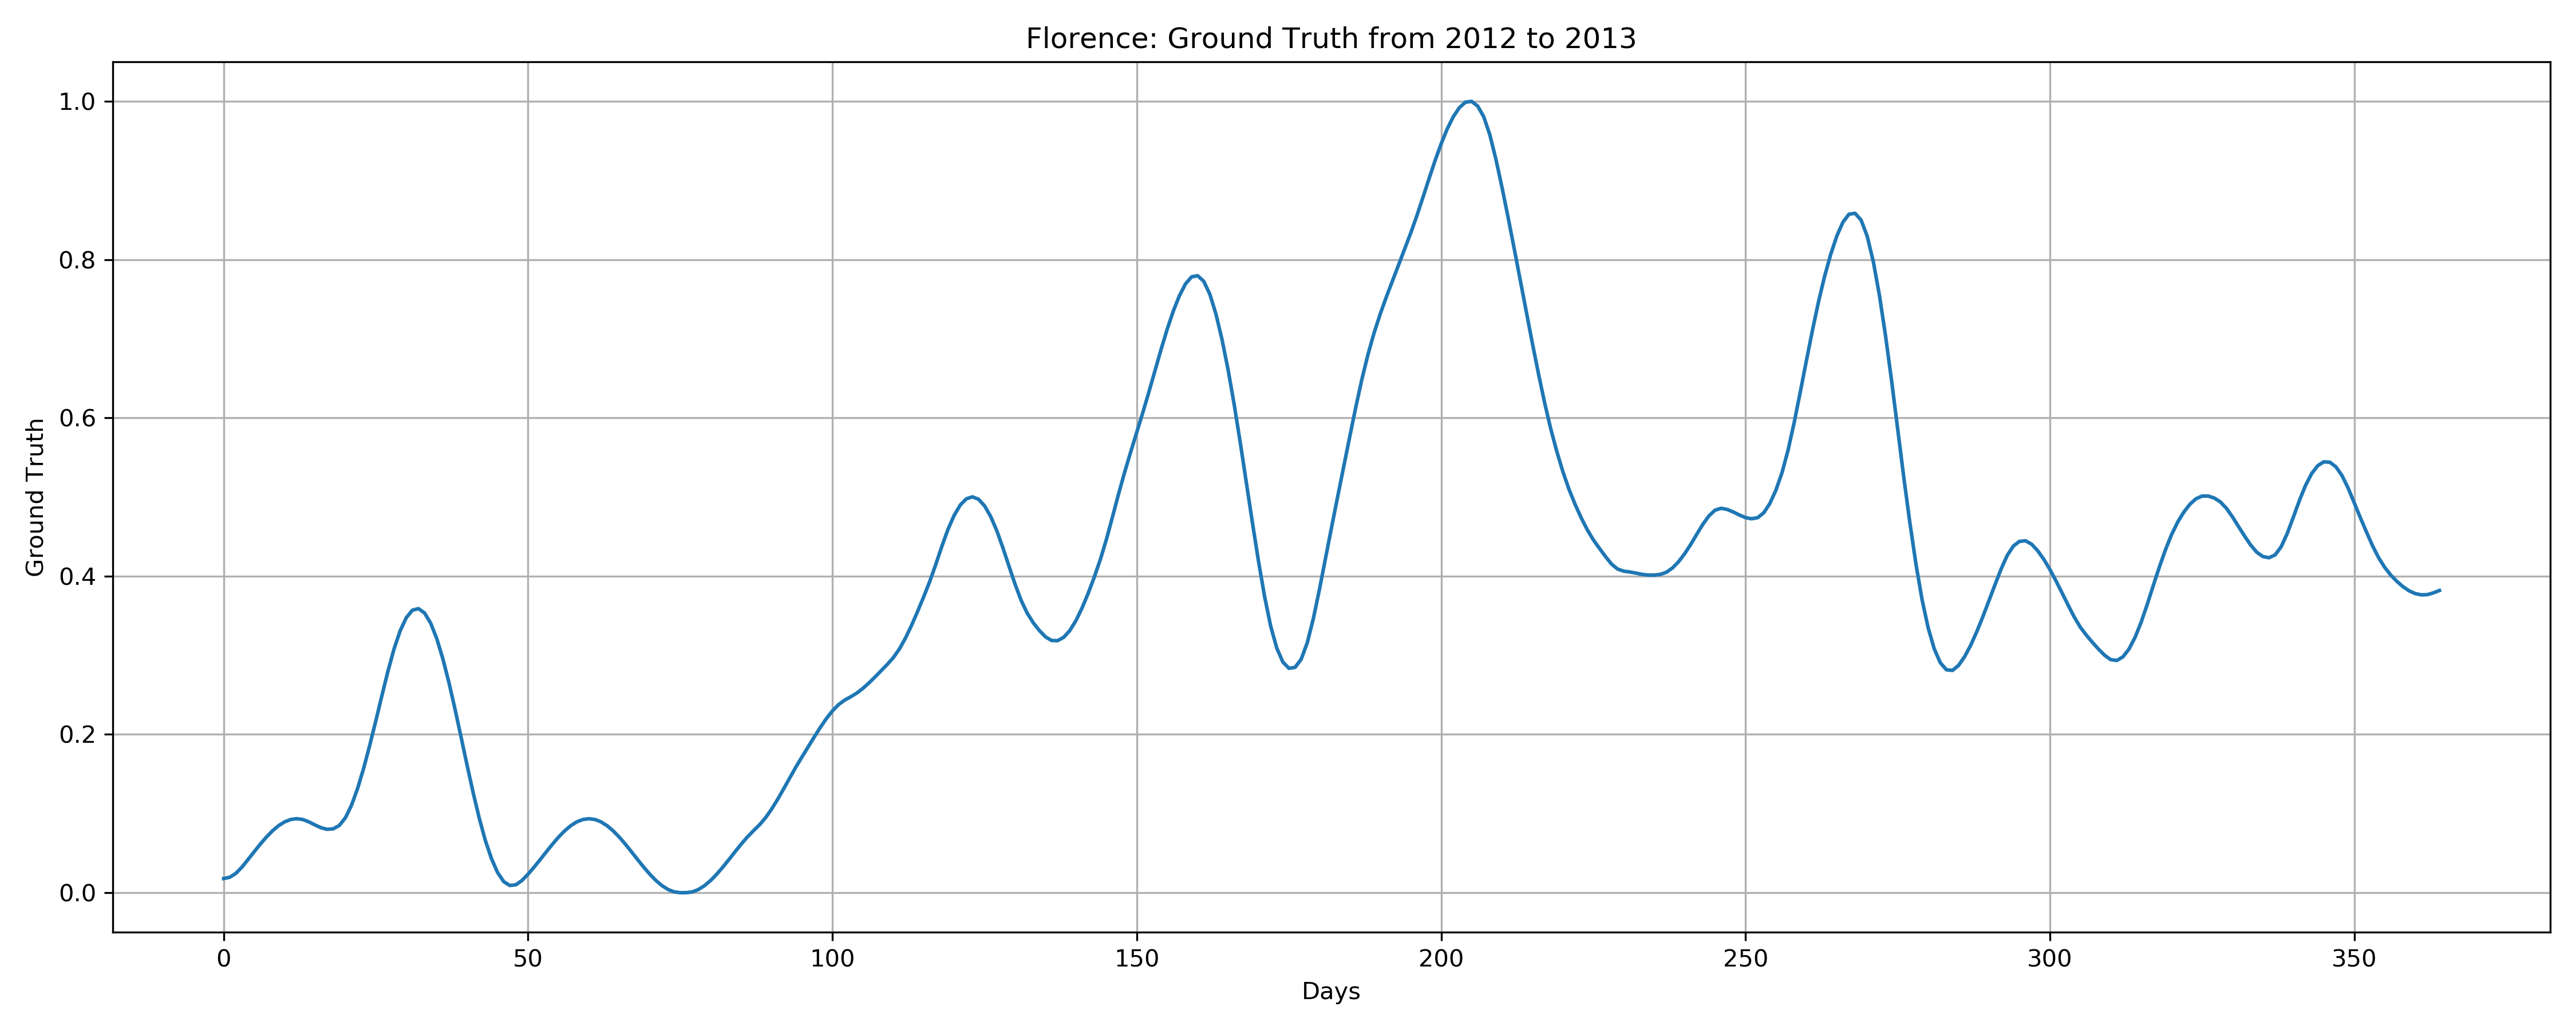
\includegraphics[width=\textwidth]{img/GT.png}}
\end{figure}
\end{frame}


\begin{frame}{Modello Data-driven}
Il problema è stato affrontato utilizzando tecniche di \textbf{Multi Task Learning}:
\begin{itemize}
    \item \textbf{Task 1}: predirre il valore di rischio del giorno successivo
    {{\scriptsize\begin{equation}\label{MAE}
    L_{MAE}(y, \hat y)=\frac{1}{N}\sum_{i=0}^N |y - \hat y|
    \end{equation}}\small} \pause
    \item \textbf{Task 2}: imparare quali finestre di osservazioni danno valori di rischio più alti
    {{\scriptsize\begin{equation}\label{MRL}
    L_{MRL}(\hat y_1, \hat y_2, z) = \max(0, -z \cdot (\hat y_1 - \hat y_2) + m)
    \end{equation}}\small}
\end{itemize}\pause
\textbf{Loss finale}:
\begin{equation}\label{custom_loss}
\mathcal{L}(L_{MRL}, L_{MAE_{1}}, L_{MAE_{2}})= L_{MRL} + \sigma(L_{MAE_{1}} + L_{MAE_{2}})
\end{equation}
dove $\sigma$ è un iperparametro del modello.
\end{frame}

\begin{frame}{Modello Data-driven}
\textbf{Architettura}:
\begin{figure}
	\centering
	\fbox{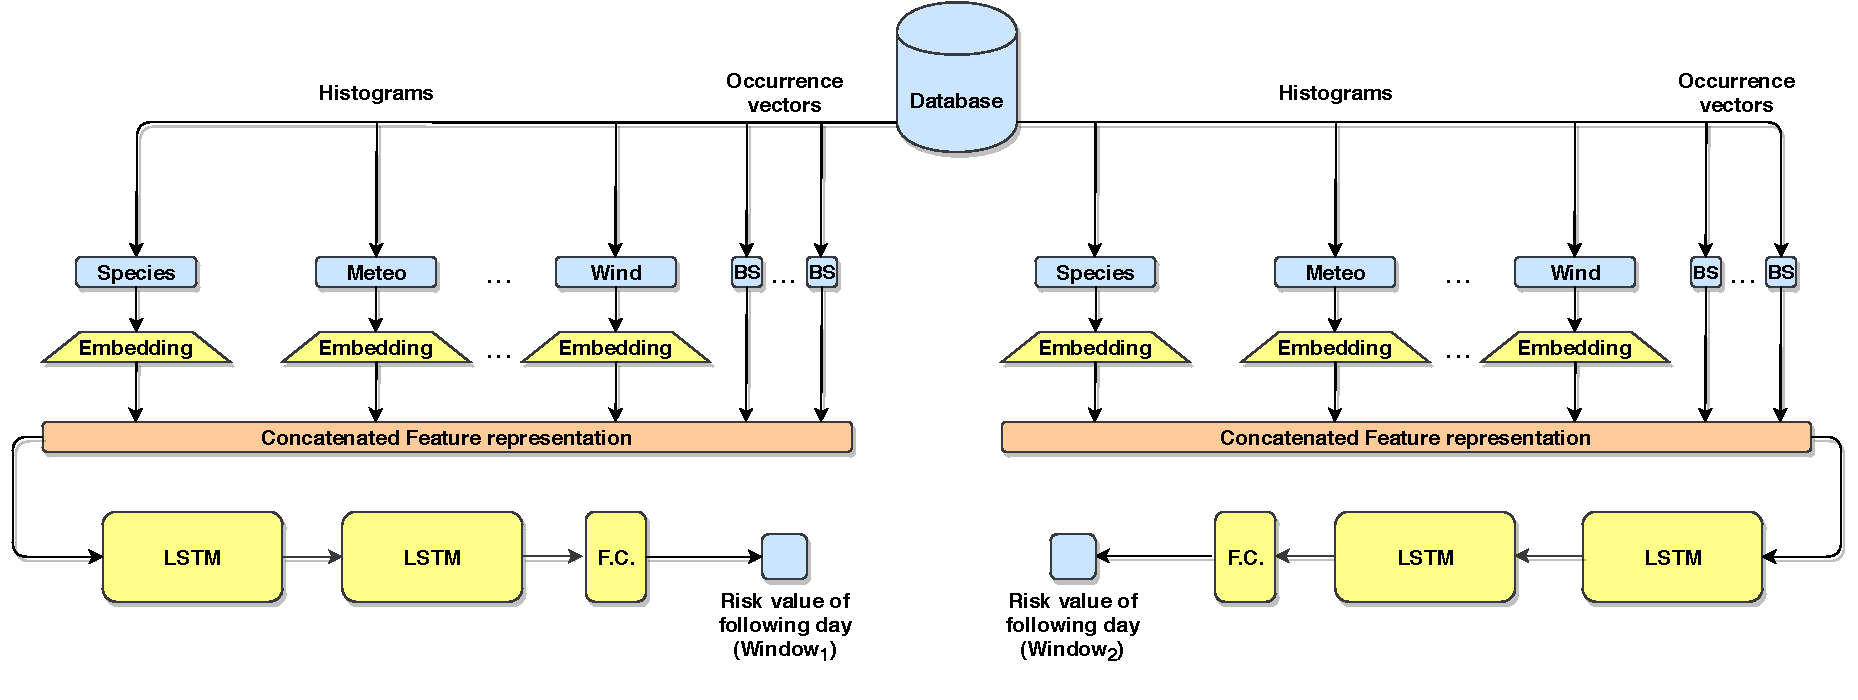
\includegraphics[width=\textwidth]{img/network3.pdf}}
\end{figure}
\end{frame}


\section{Risultati sperimentali}
\begin{frame}{Risultati sperimentali}

Il modello è stato testato su \textbf{8 aereoporti}.
Il dataset comprede dati \textbf{dal 2012 al 2018}:
\begin{itemize}
    \item 1852 giorni per il training
    \item 575 giorni per il testing
\end{itemize}

La metrica utilizzata per la valutazione è la correlazione di Spearman.


\end{frame}

\begin{frame}{Risultati sperimentali}
\textbf{Risultati}

\begin{table}
\centering
\scalebox{0.82}{
\begin{tabular}{@{}ccc@{}}
	\toprule
	Aeroporto & Modello Proposto & $BRI_2$ \\ 	\midrule
	Firenze & \textbf{0.83} & 0.17\\
	Pisa & \textbf{0.84} & 0.47\\
	Bologna & \textbf{0.86} & 0.26\\
	Milano-Malpensa &  \textbf{0.82} & -0.14\\
	Milano-Linate &  \textbf{0.94} & -0.28\\
	Verona & \textbf{0.87} & 0.60\\
    Catania & \textbf{0.86} & 0.49\\
    Brescia & -0.20 & 0.31\\    \bottomrule
\end{tabular}}
\end{table}

\end{frame}

\begin{frame}{Risultati sperimentali}
\textbf{Esempio di risultato qualitativo: Aeroporto di Firenze}
\begin{figure}
	\centering
	\fbox{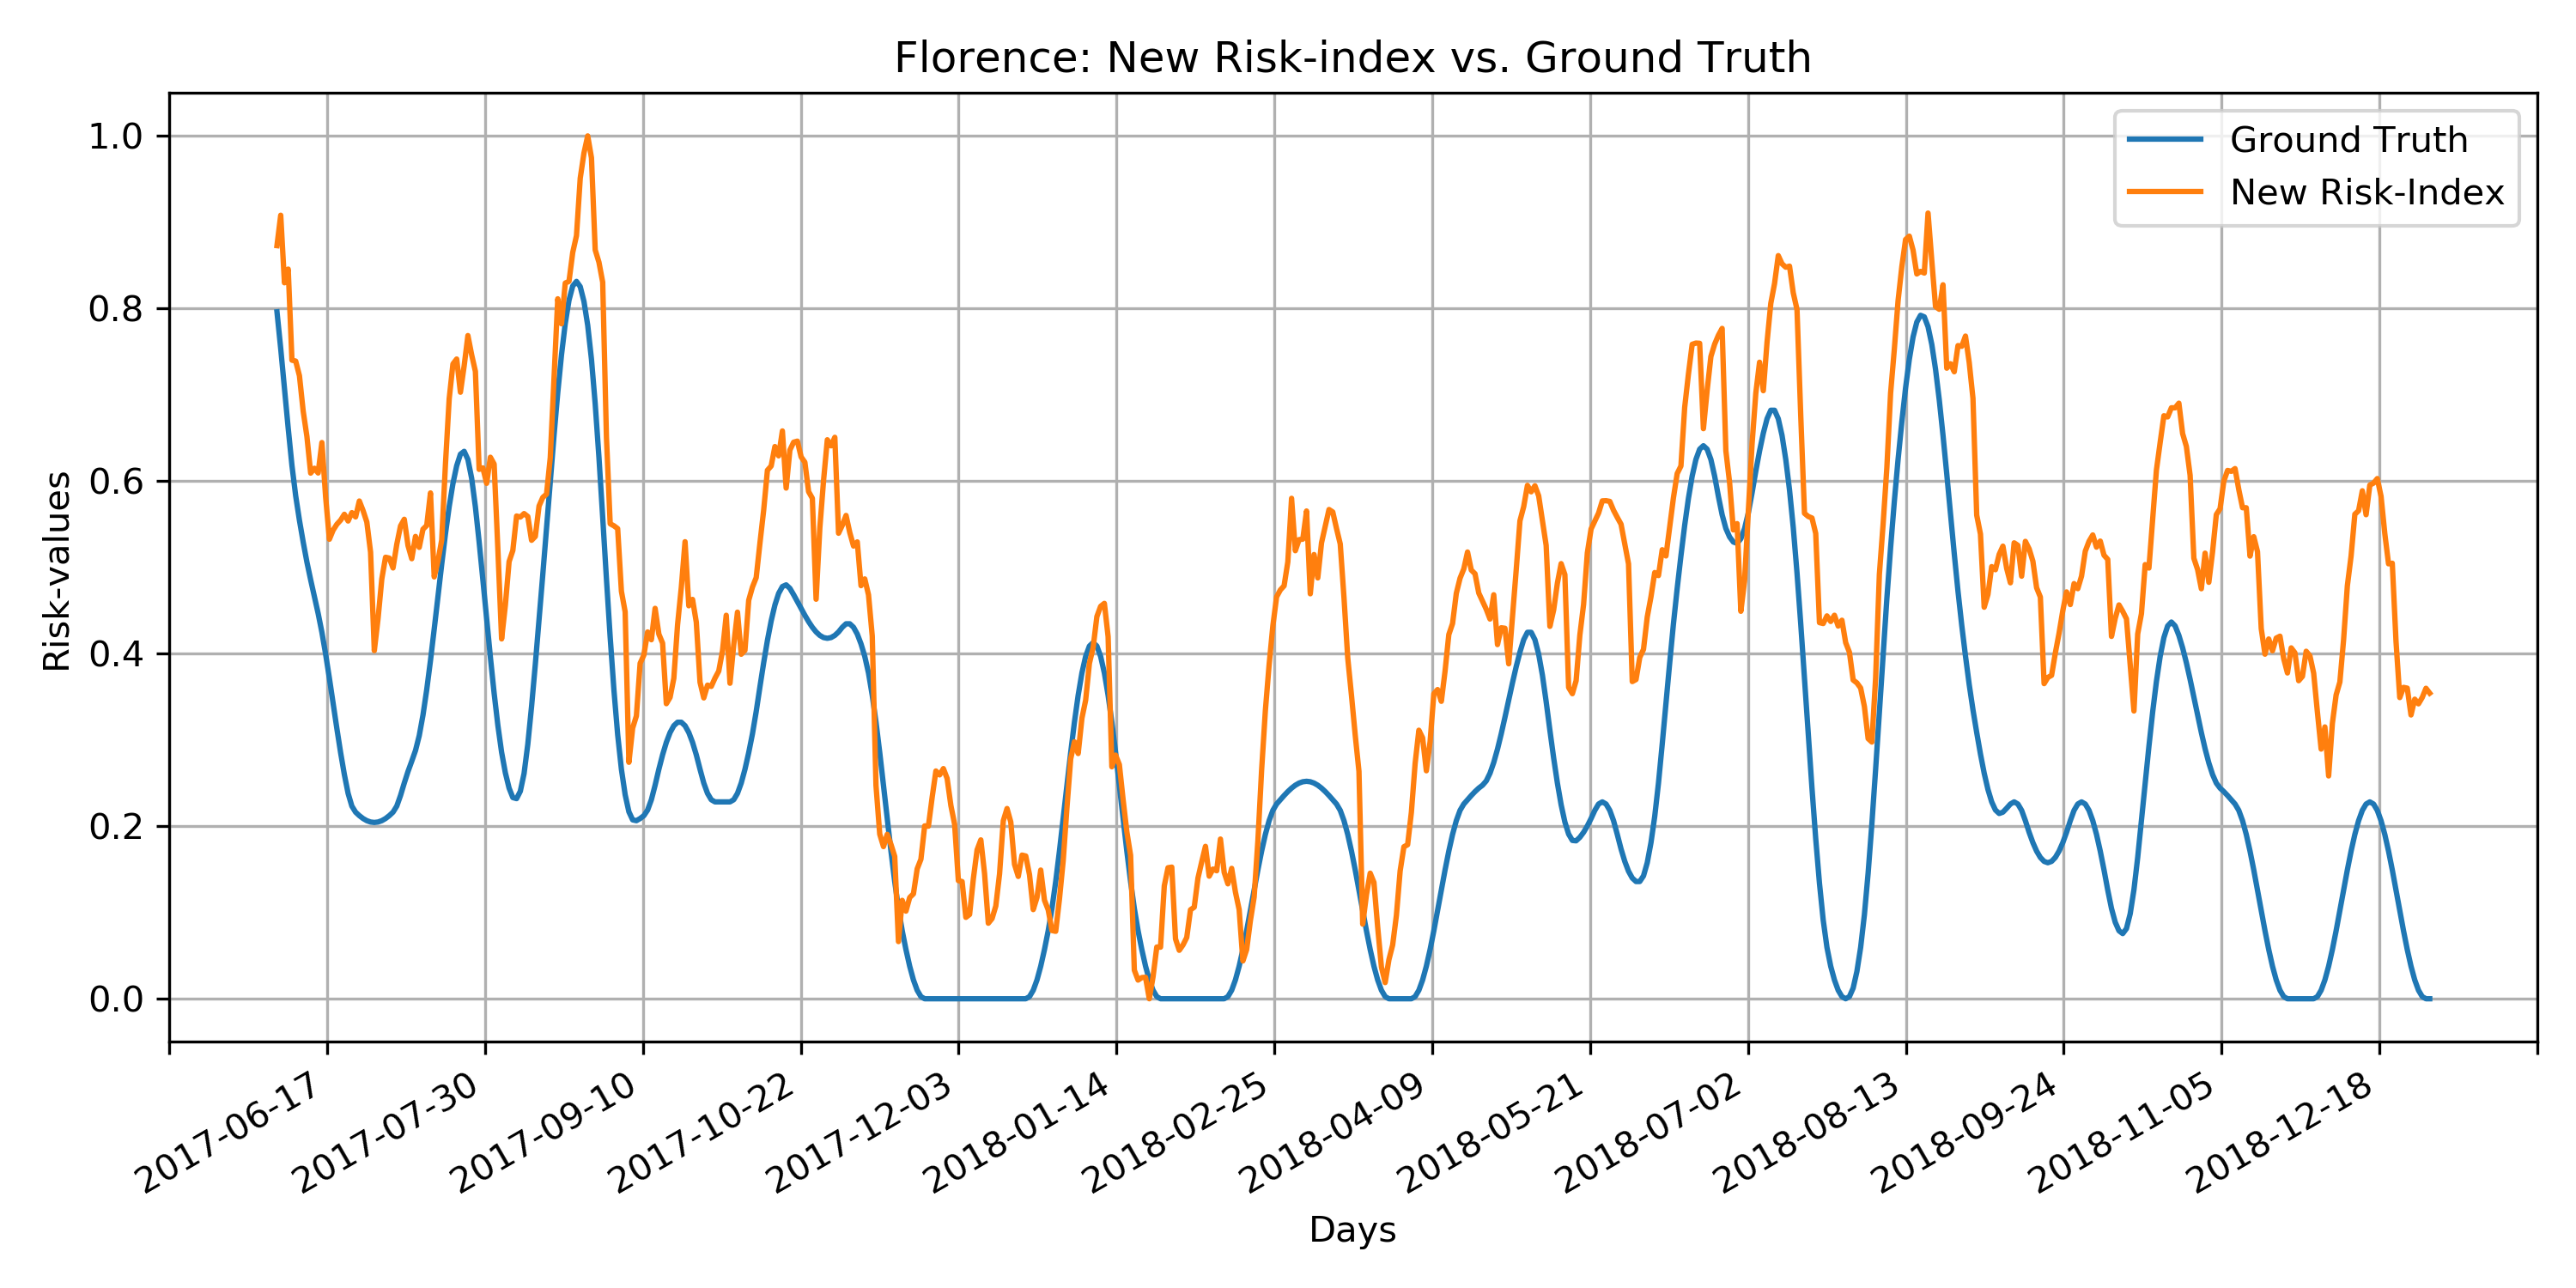
\includegraphics[width=\textwidth]{img/FI.png}}
\end{figure}
\end{frame}

\begin{frame}{Risultati sperimentali}
\textbf{Esempio di risultato qualitativo: Aeroporto di Verona}
\begin{figure}
	\centering
	\fbox{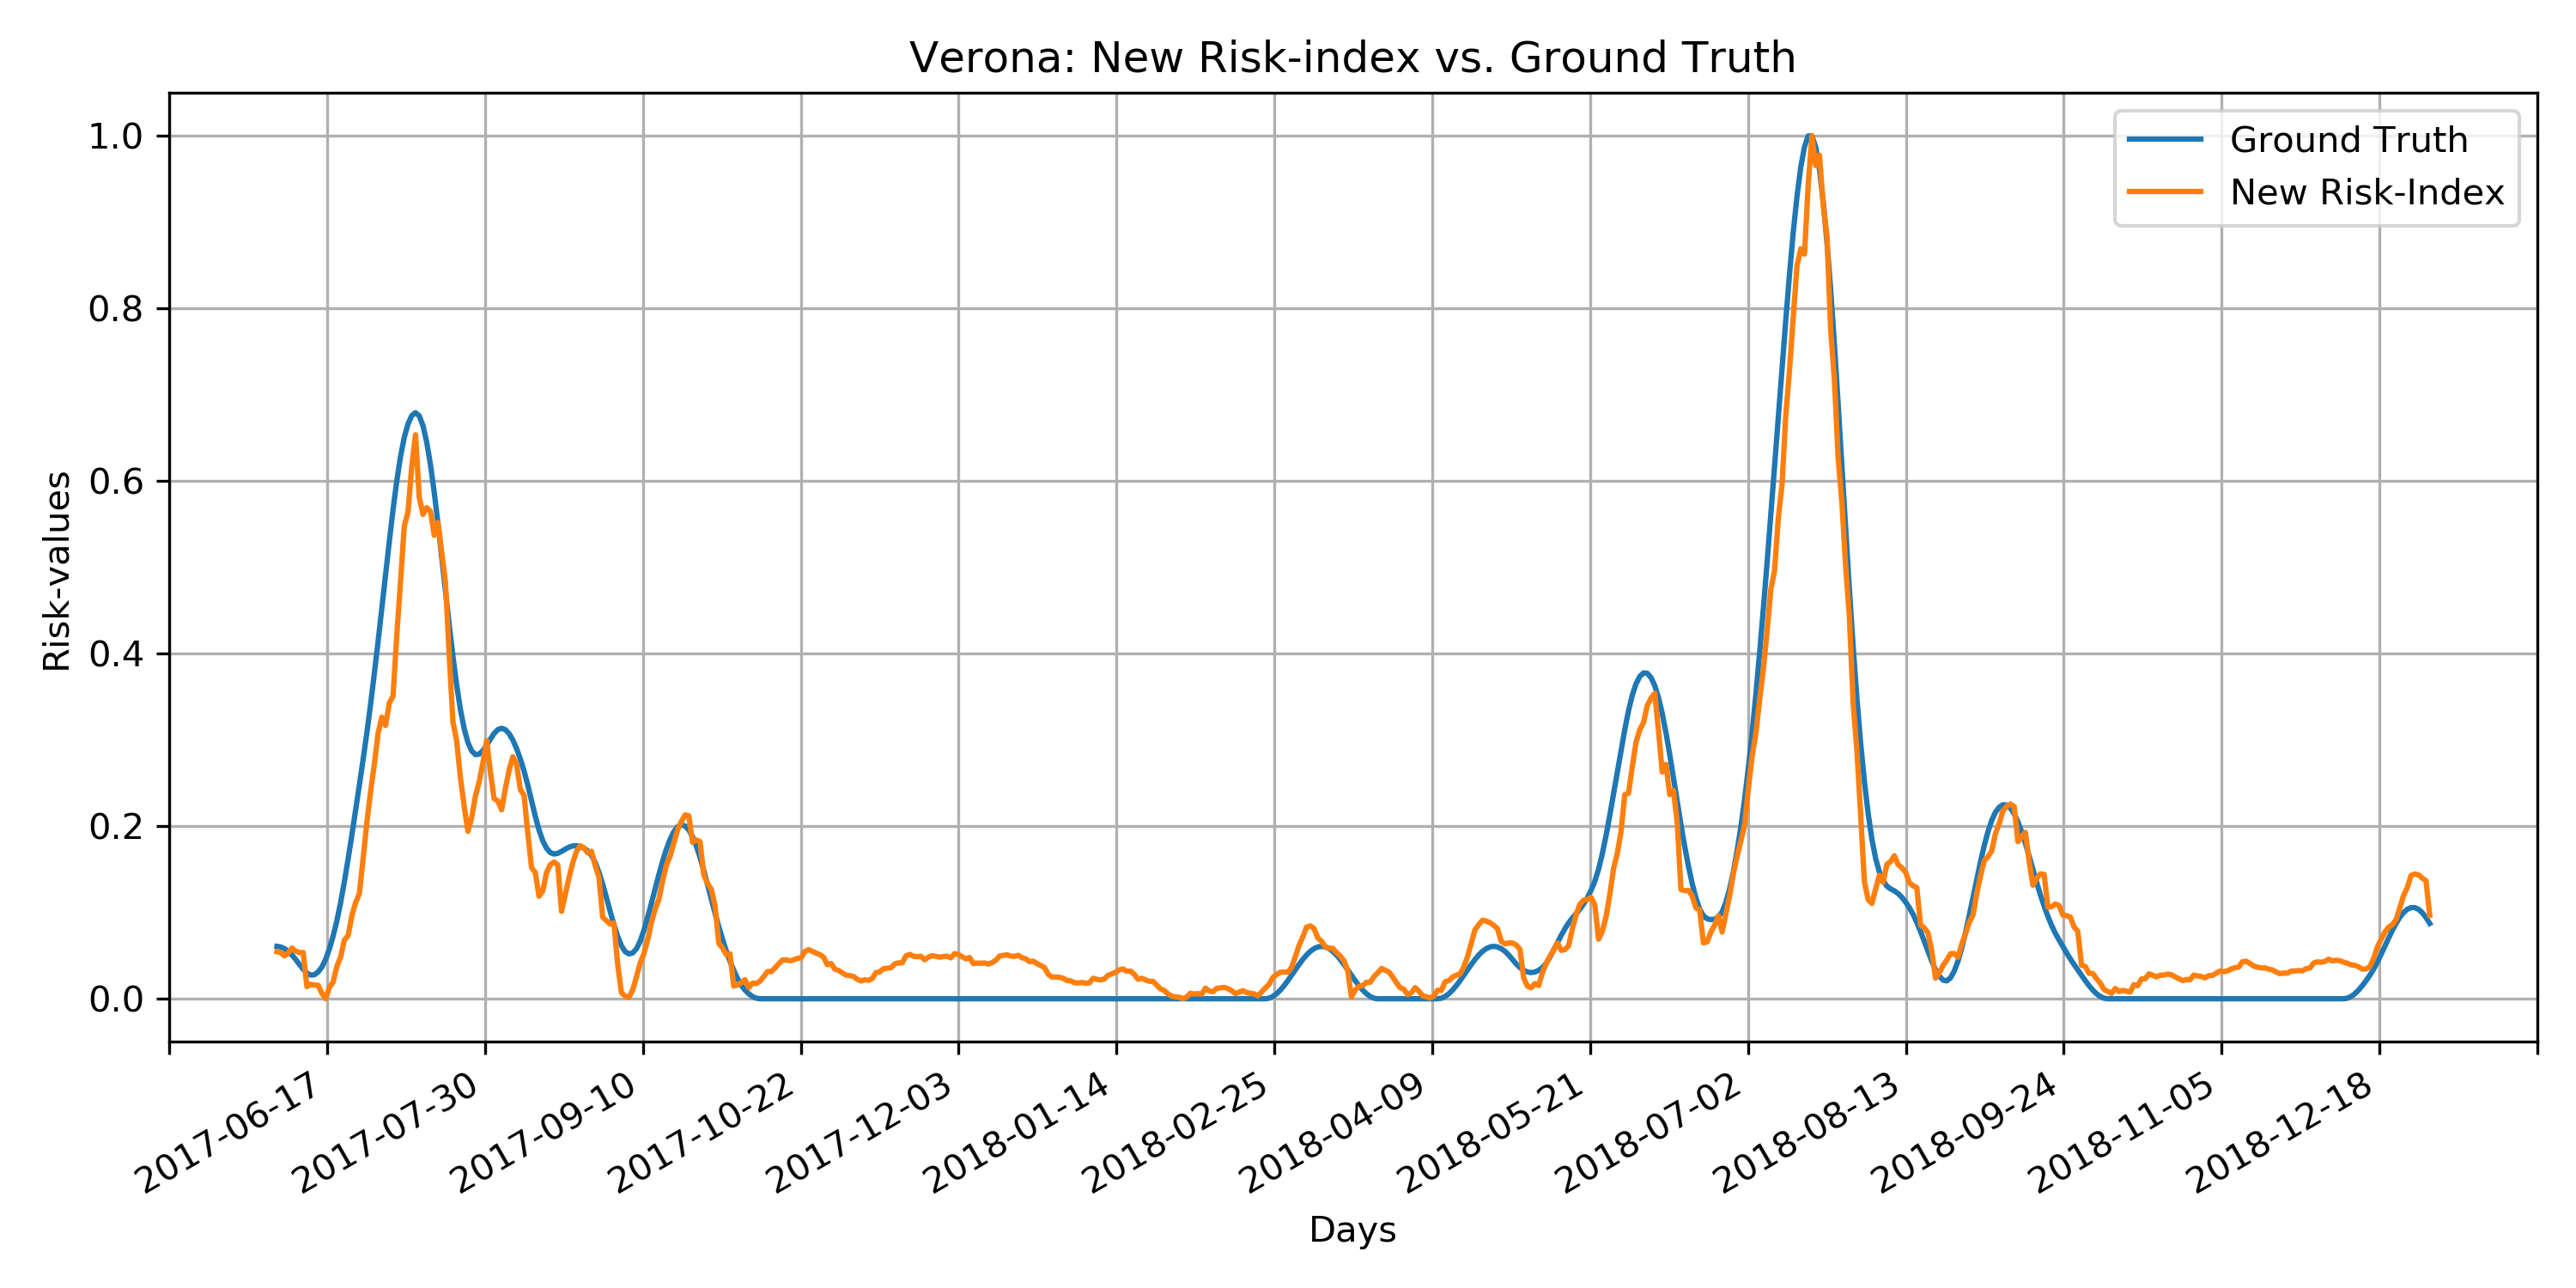
\includegraphics[width=\textwidth]{img/VE.png}}
\end{figure}
\end{frame}

\begin{frame}{Risultati sperimentali}
\textbf{Confronto tra modelli testati:}
\begin{figure}
	\centering
	\fbox{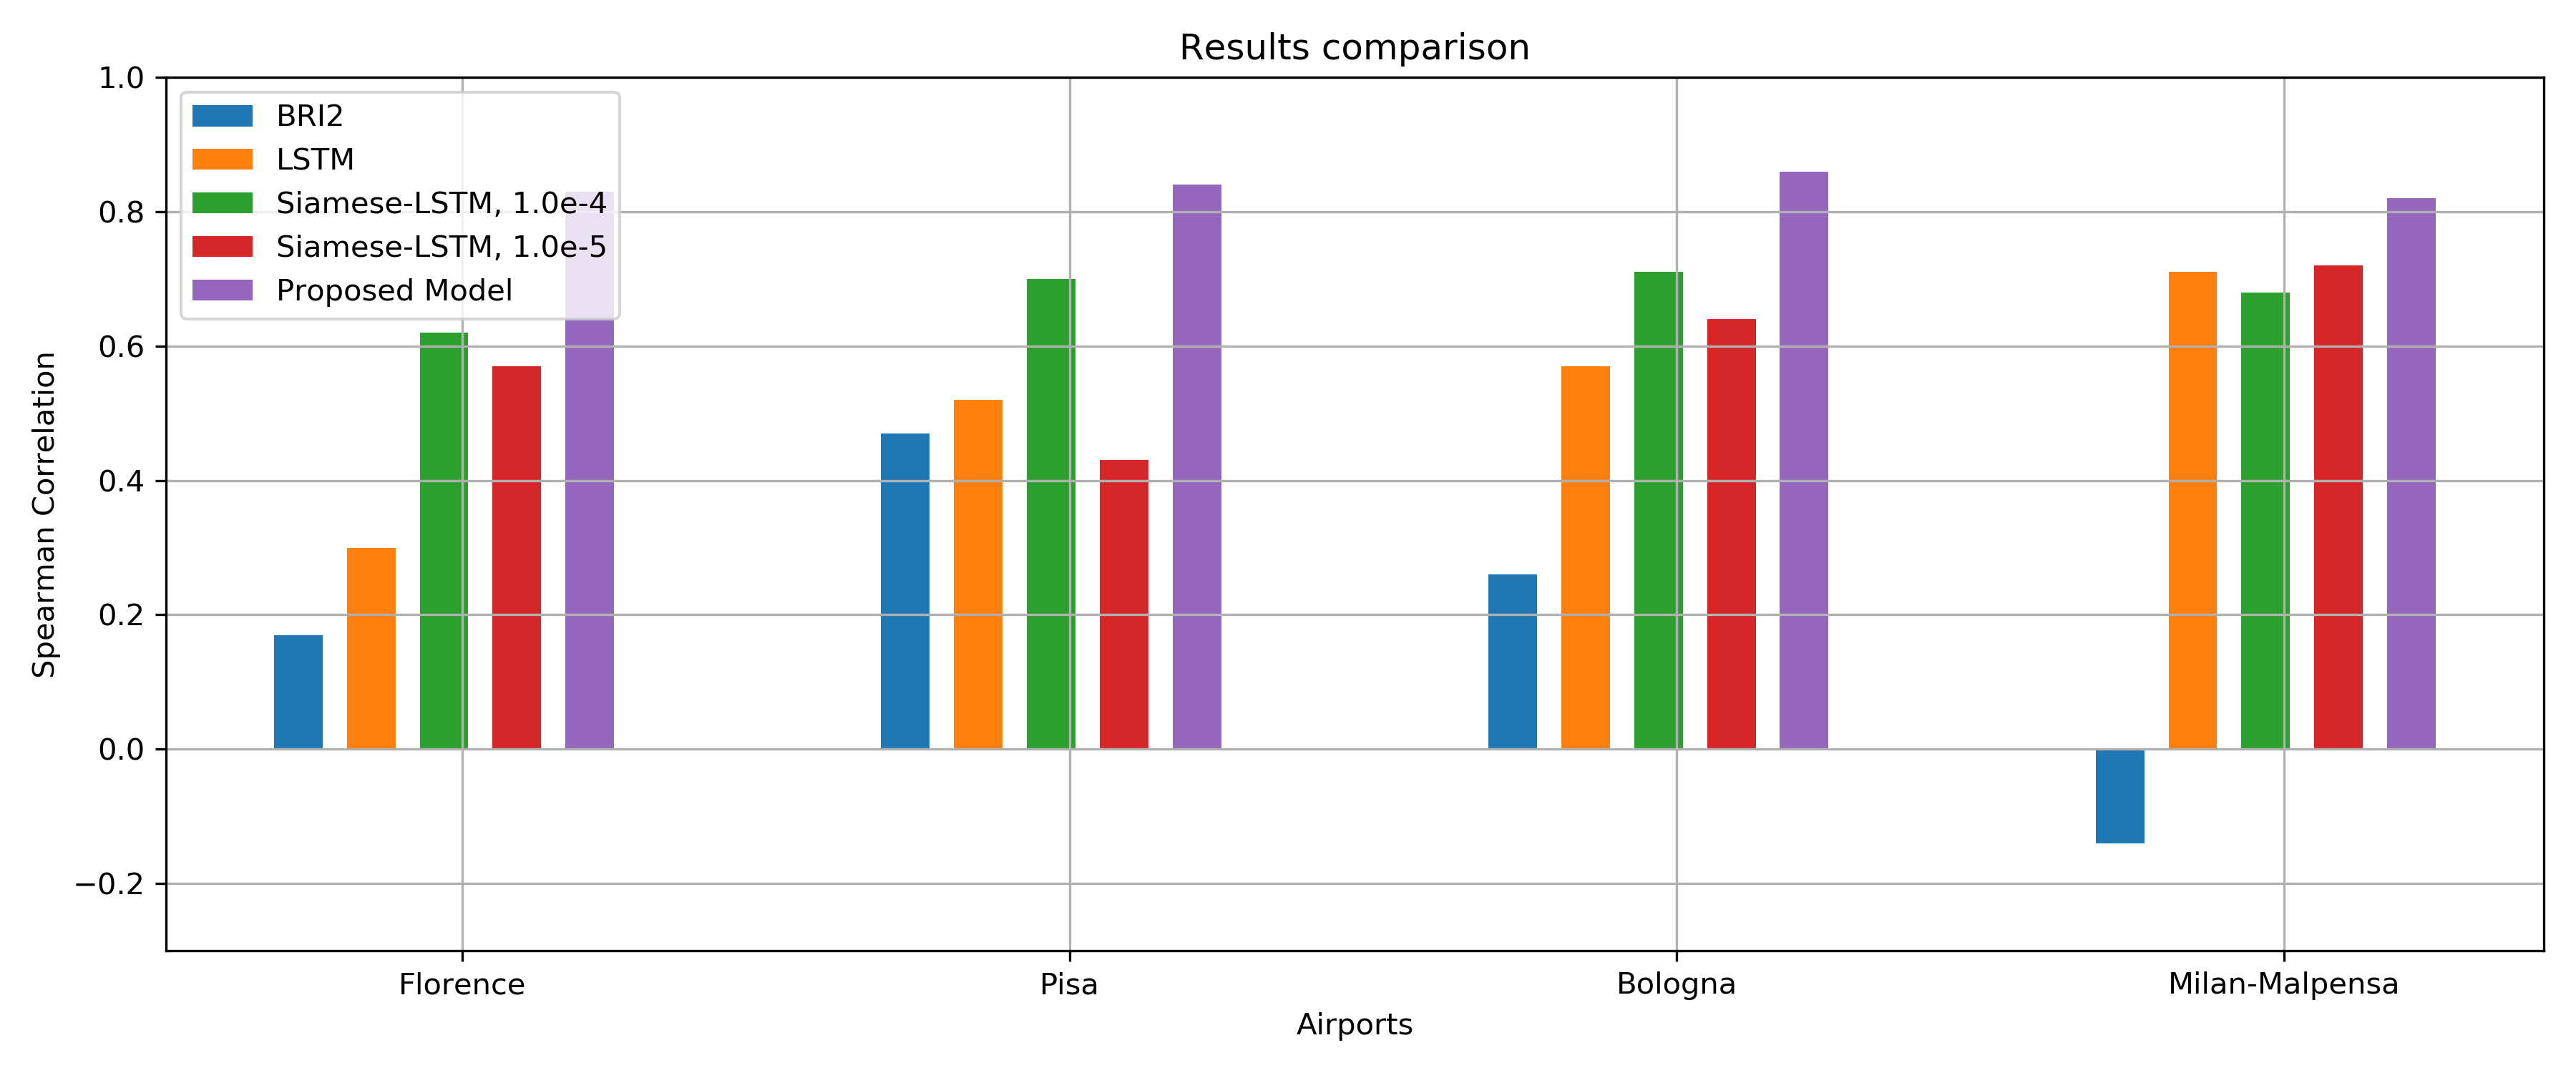
\includegraphics[width=8cm]{img/comparison1.png}}\par
	\fbox{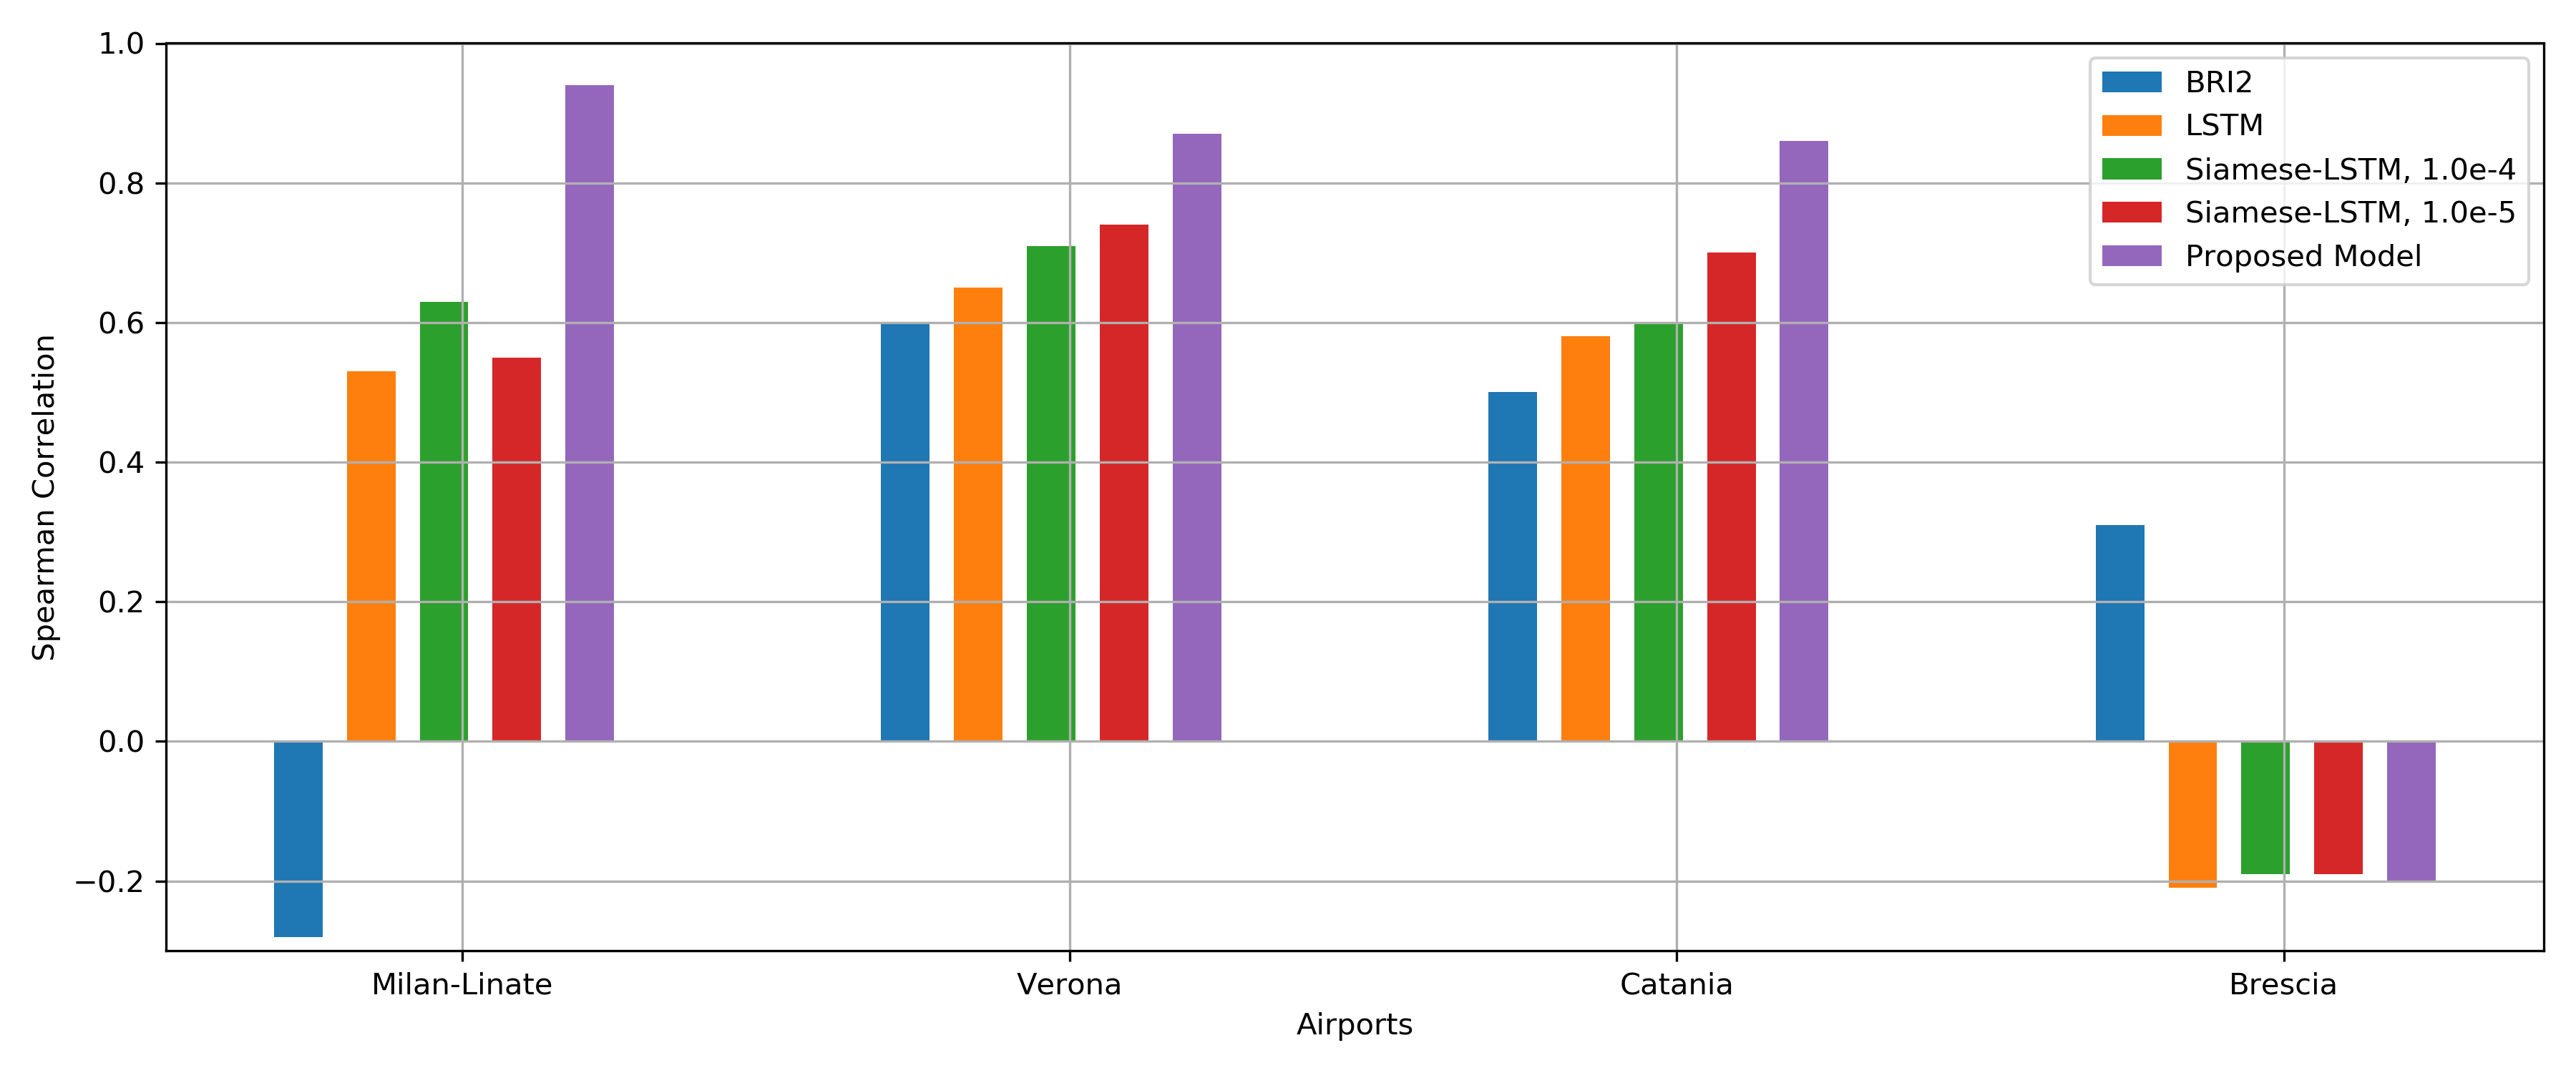
\includegraphics[width=8cm]{img/comparison2.png}}
\end{figure}
\end{frame}

\section{Conclusioni}
\begin{frame}{Conclusioni e sviluppi futuri}
\textbf{Conclusioni:}\par
Il modello data-driven proposto:
\begin{itemize}
    \item \`E un affidabile predittore di rischio
    \item Fornisce un valore di rischio giornaliero
    \item Ha raggiunto ottimi risultati per il sottoinsieme degli aeroporti scelti
    \item\`E fortemente correlato agli eventi di birdstrike
    \item Ha una migliore correlazione rispetto al $BRI_2$
\end{itemize}

\textbf{Sviluppi futuri:}
\begin{itemize}
    \item Testare il modello su ulteriori aeroporti 
    \item Ottenere il numero di voli giornaliero ed aggiungerlo alle feature
    \item Introdurre una soglia di rischio
\end{itemize}
\end{frame}

\begin{frame}{Ringraziamenti}
Ringrazio \textbf{Magenta S.r.l}. per il contributo a questo lavoro di tesi e \textbf{Birdcontrol Italy S.r.l.} che ha fornito il dataset utilizzato che comprende 10+ anni di monitoraggio nei principali aeroporti Italiani.
\end{frame}

\maketitle

\end{document}
